\documentclass[12pt, a4paper]{article}
\input{/home/mykhailo/.config/nvim/templates/preamble.tex}

\newcommand{\department}{ЗІ}
\newcommand{\reportnumber}{4}
\newcommand{\reporttitle}{Робота з JavaScript}
\newcommand{\profname}{Синявський О. Ю.}

\begin{document}

\input{/home/mykhailo/Documents/lpnu/report_title_page}
\section{Частина 1: робота з JavaScript}
Мета --- Засвоїти базові концепції JavaScript та навчитися керувати потоком виконання програми. Ознайомитися з основами взаємодії JavaScript з HTML.
\subsection{Хід роботи}
\begin{enumerate}
	\item Зберігання даних у браузері
		\begin{itemize}
			\item Зберегти всю наявну інформацію про операційну систему та браузер у \verb|localStorage|.
			\item Відобразити всю наявну інформацію у \verb|localStorage| у футері сайту.
		\end{itemize}
	\item Відображення динамічного вмісту отриманого із сервера
		\begin{itemize}
			\item Зробити запит на сервер для відображення коментарів ваших попередніх роботодавців.
			\item Для отримання вигаданих коментарів потрібно скористатись безкоштовним ресурсом \textbf{JSONPlaceholder - Free Fake REST API}. А саме \verb|jsonplaceholder.typicode.com/post/11/comments| 
			\item Відобразити отримані коментарі у порядку їх отримання.
		\end{itemize}
	\item Надсилання форми зворотного зв'язку
		\begin{itemize}
			\item Після того як користувач пробуде на сайті 1 хвилину, нам потрібно показати йому модальне вікто із формою зворотного зв'язку.
			\item Форма має містити такі поля:
				\begin{itemize}
					\item Ім'я
					\item Email
					\item Номер телефону
					\item Поле для тексту у довільній формі
					\item Кнопка "Надіслати"
				\end{itemize}
			\item Після натискання на кнопку "Надіслати", форма має надсилатися на електронну пошту студента.
			\item Зареєструйтесь на сайті Formspree. Ця платформа дозволяє надсилати до 50 листів на місяць безкоштовно без жодної конфігурації вашого власного сервера.
			\item Створіть нову форму (отримайте унікальний endpoint для обробки).
			\item Змініть тег \verb|<form>| у своєму HTML, на щось подібне: \verb|<form action="https://formspree.io/f/..." method="POST">|. Це дозволить надіслати дані на сервер, який уже обробить цей запит і надішле вам електронного листа із вмістом форми.
		\end{itemize}
	\item Перехід на нічний/денний режим
		\begin{itemize}
			\item Додати перемикач на сторінку, який перемикатиме денну та нічну тему сайту.
			\item Додати функціональність, яка залежно від часу доби буде автоматично перемикати тему сайту.
				\begin{itemize}
					\item Денна тема: від 07:00 до 21:00.
					\item Нічна тема: в увесь інший час.
				\end{itemize}
		\end{itemize}
\end{enumerate}
\subsection{Лістинг}
\begin{lstlisting}
<!DOCTYPE html>
<html>
	<head>
		<title>JS</title>
		<style>
			body, dialog {
				background-color: #fff;
				color: #000;
				transition: background-color 0.3s ease, color 0.3s ease;
			}

			body.dark-mode, dialog.dark-mode {
				background-color: #000;
				color: #fff;
			}
		</style>
	</head>
	<body>
		<button id="themeSwitch">Switch to dark mode</button>
		<div id="commentContainer">
			<p>Comments:</p>
		</div>
		<footer id="dynamicFooter"></footer>
		<dialog id="contactDialog">
			<form method="POST" id="contactForm" action="https://formspree.io/f/mjyyazby">
				<label for="nameInput">Name: </label>
				<input type="text" id="nameInput" name="name"/>
				<br/>
				<label for="emailInput">Email: </label>
				<input type="email" id="emailInput" name="email"/>
				<br/>
				<label for="phoneInput">Phone number: </label>
				<input type="tel" id="phoneInput" name="phoneNumber"/>
				<br/>
				<label for="paragraphInput">Message: </label>
				<textarea id="paragraphInput" rows="5" cols="40" name="messageBody"></textarea>
				<br/>
				<input type="submit" value="Contact me!"/>
			</form>
		</dialog>
		<script>
			const sysInfo = {
				userAgent: navigator.userAgent,
				platform: navigator.platform,
			}
			localStorage.setItem('sysInfo', JSON.stringify(sysInfo))
			
			const footer = document.getElementById('dynamicFooter')
			const commentContainer = document.getElementById("commentContainer")
			const dialog = document.getElementById('contactDialog')
			setTimeout(() => {
				dialog.showModal();
			}, 60000);
			footer.textContent = sysInfo.userAgent + "; " + sysInfo.platform
		
			try {
				fetch('https://jsonplaceholder.typicode.com/posts/11/comments')
					.then(response => {
						if(!response.ok) {
							throw new Error(`HTTP error! Status: ${response.status}`)
						}

						return response.json();
					})
					.then(data => {
						console.log(data)
						data.forEach((comment, index) => {
							const commentCard = document.createElement('div')
							commentCard.innerHTML = `
								<h3>${comment.name}</h3>
								<h4>${comment.email}</h4>
								<p>${comment.body}</p>
							`
							commentContainer.appendChild(commentCard)
						})
					})
			} catch (error) {
				console.error('Failed to fetch comments:', error)
			}

			let form = document.getElementById('contactForm')
			async function handleSubmit(event) {
				console.log("fired")
				event.preventDefault();
				let data = new FormData(event.target);

				fetch(event.target.action, {
					method: form.method,
					body: data,
					headers: {
						'Accept': 'application/json'
					}
				}).then(response => {
					if(response.ok) {
						form.reset();
						dialog.close()
					}
				}).catch(error => {
					console.error(error)
				})
			}
			form.addEventListener('submit', handleSubmit);

			const currentHour = new Date().getHours();
			const themeSwitch = document.getElementById('themeSwitch')
			let isWhiteTheme = currentHour >= 7 && currentHour <= 21;

			if(!isWhiteTheme) {
				document.body.classList.add('dark-mode');
				contactDialog.classList.add('dark-mode');
				themeSwitch.textContent = 'Switch to light mode'
			}

			themeSwitch.addEventListener('click', () => {
				document.body.classList.toggle('dark-mode')
				contactDialog.classList.toggle('dark-mode');

				if(document.body.classList.contains('dark-mode')) {
					themeSwitch.textContent = "Switch to light mode"
				} else {
					themeSwitch.textContent = "Switch to dark mode"
				}
			})
		</script>
	</body>
</html>
\end{lstlisting}
\section{Частина 2: реалізація в React}
Мета --- Застосувати вивчені концепції JavaScript у середовищі React. Ви реалізуєте ті самі функції, що й у частині 1, але використовуючи хуки React (\verb|useState|, \verb|useEffect|) та компоненти у вашому проєкті \verb|lab_2_react|. 
\subsection{Хід роботи}
\begin{enumerate}
	\item Системна інформація у футері
		\begin{itemize}
			\item Завдання: Оновіть ваш компонент \verb|Footer|, щоб він відображав системну інформацію.
			\item Реалізація:
				\begin{itemize}
					\item Використовуйте хук \verb|useEffect|, щоб зчитати \verb|navigator.userAgent| та \verb|navigator.platform|, коли компонент монтується.
					\item Збережіть ці дані в \verb|localStorage| всередині ефекту.
					\item Отримайте дані з \verb|localStorage| та відобразіть їх у JSX компонента \verb|Footer|.
				\end{itemize}
		\end{itemize}
	\item Отримання відгуків
		\begin{itemize}
			\item Завдання: Створіть новий компонент з назвою \verb|Reviews.jsx|.
			\item Реалізація:
				\begin{itemize}
					\item Використовуйте \verb|useEffect|, щоб отримати дані з \verb|https://jsonplaceholder.typicode.com/|
					\verb|posts/11/comments|.
					\item Використовуйте \verb|useState| для збереження списку отриманих коментарів.
					\item Відрендеріть коментарі, використовуючи метод \verb|.map()|, щоб створити список карток відгуків.
					\item Імпортуйте та додайте компонент \verb|Reviews| у ваш \verb|App.jsx|.
				\end{itemize}
		\end{itemize}
	\item Модальне вікно форми зворотного зв'язку
		\begin{itemize}
			\item Завдання: Створіть компонент \verb|ContactForm.jsx|, який відкриває модальне вікно.
			\item Логіка модального вікна: 
				\begin{itemize}
					\item Створіть змінну стану \verb|isOpen| (початково \verb|false|).
					\item Використовуйте \verb|useEffect| з \verb|setTimeout|, щоб встановити \verb|isOpen| в \verb|true| через 1 хвилину.
					\item Додайте кнопку "Закрити" в модальне вікно, щоб встановити \verb|isOpen| назад в \verb|false|.
				\end{itemize}
			\item Реалізація форми:
				\begin{itemize}
					\item Форма повинна містити ті самі поля, що й у частині 1 (Ім'я, Email, Телефон, Повідомлення).
					\item Використовуйте ту саму URL-адресу дії Formspree, яку ви створили в частині 1.
					\item Ви можете використовувати стандартний тег \verb|<form>| з \verb|action="..." method="POST"|.
				\end{itemize}
		\end{itemize}
	\item Розумний перемикач теми
		\begin{itemize}
			\item Завдання: Реалізуйте перемикач темної/світлої теми з \verb|App.jsx| або провайдері контексту.
			\item Вимоги:
				\begin{itemize}
					\item Створіть змінну стану \verb|theme|.
					\item Автоматичне перемикання: При початковому завантаженні (\verb|useEffect|), перевірте поточний час. Якщо зараз між 07:00 та 21:00, встановіть \verb|theme| в \verb|'light'|, інакше в \verb|'dark'|.
					\item Ручне перемикання: Додайте кнопку в шапці/навігації для ручного перемикання між режимами.
					\item Застосування стилів: Використовуйте стан \verb|theme|, щоб застосувати CSS-клас \verb|'dark'| з Tailwind до елемента \verb|<body>| або вашої головної обгортки застосунку.
				\end{itemize}
		\end{itemize}
\end{enumerate}
\subsection{Результат}
\begin{figure}[H]
	\centering
	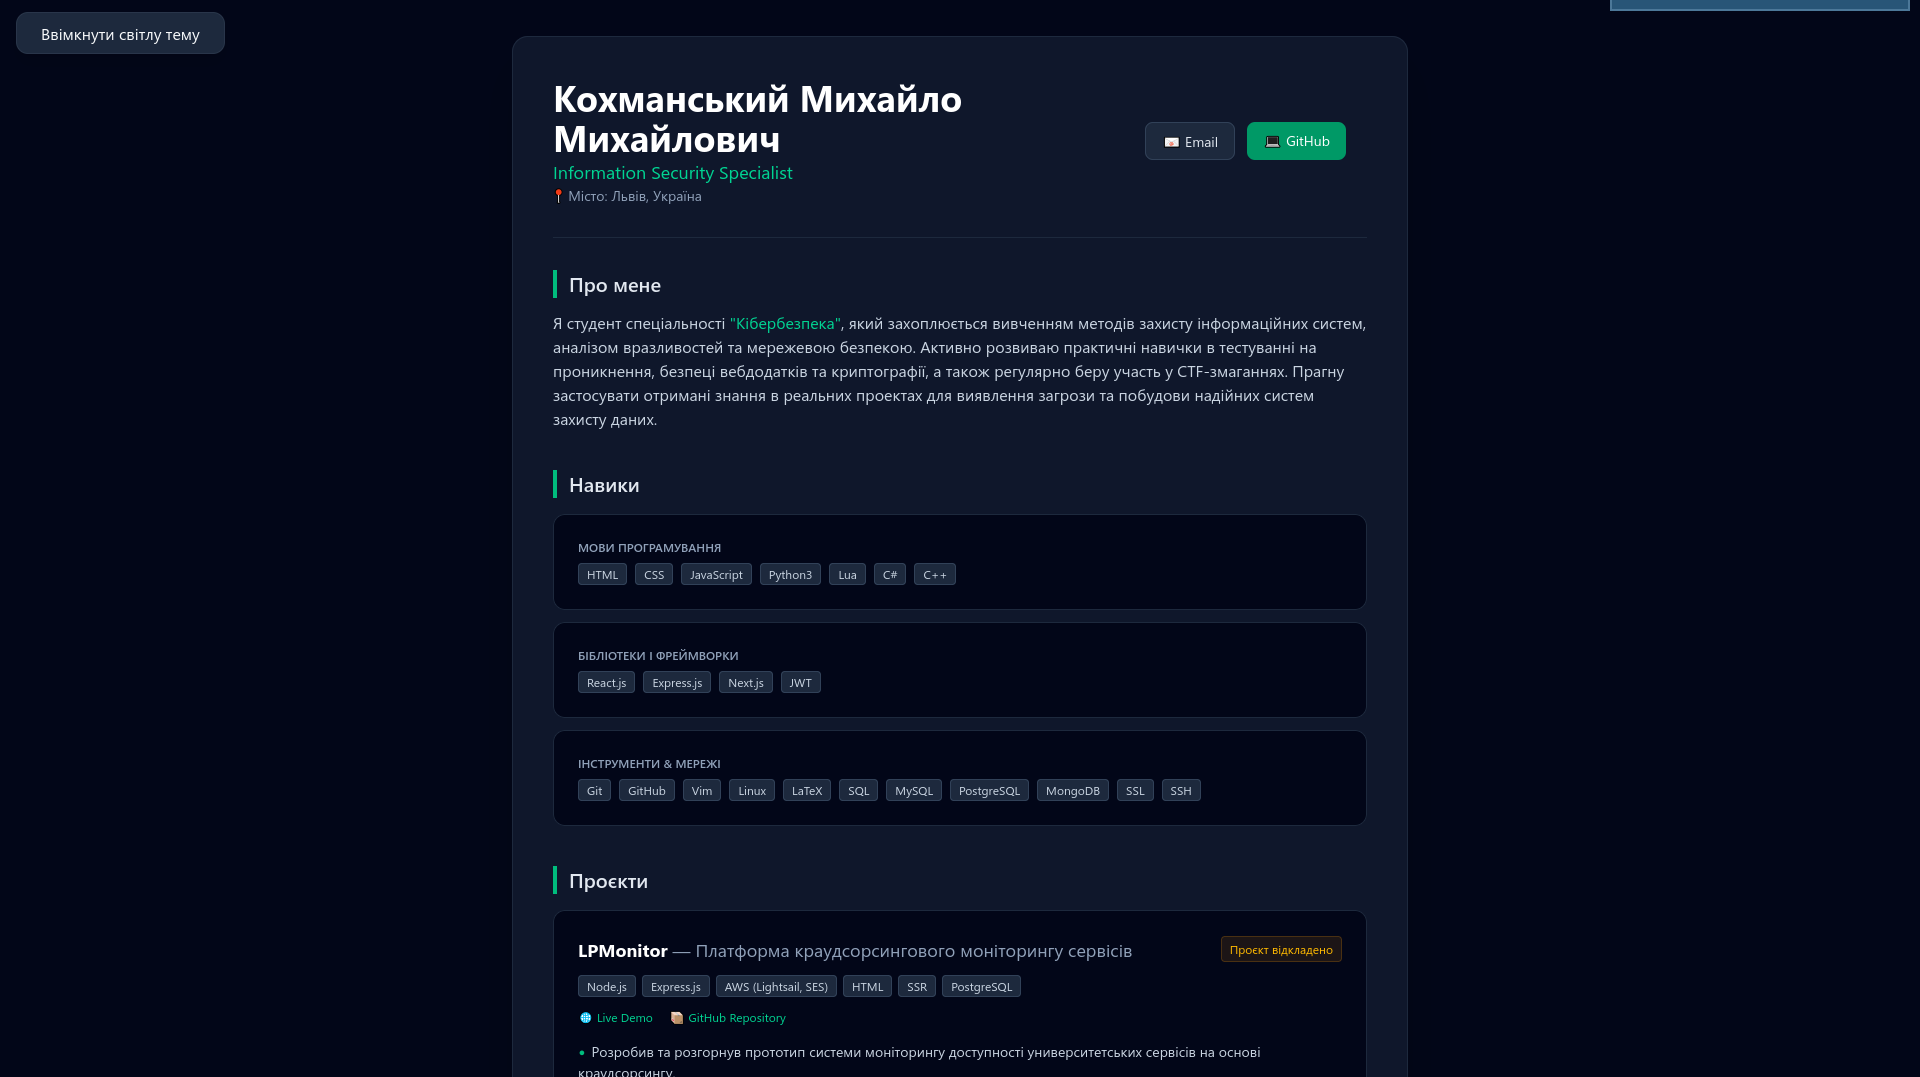
\includegraphics[width=0.7\textwidth]{result_dark.png}
	\caption{Вигляд сторінки з темною темою}
\end{figure}
\begin{figure}[H]
	\centering
	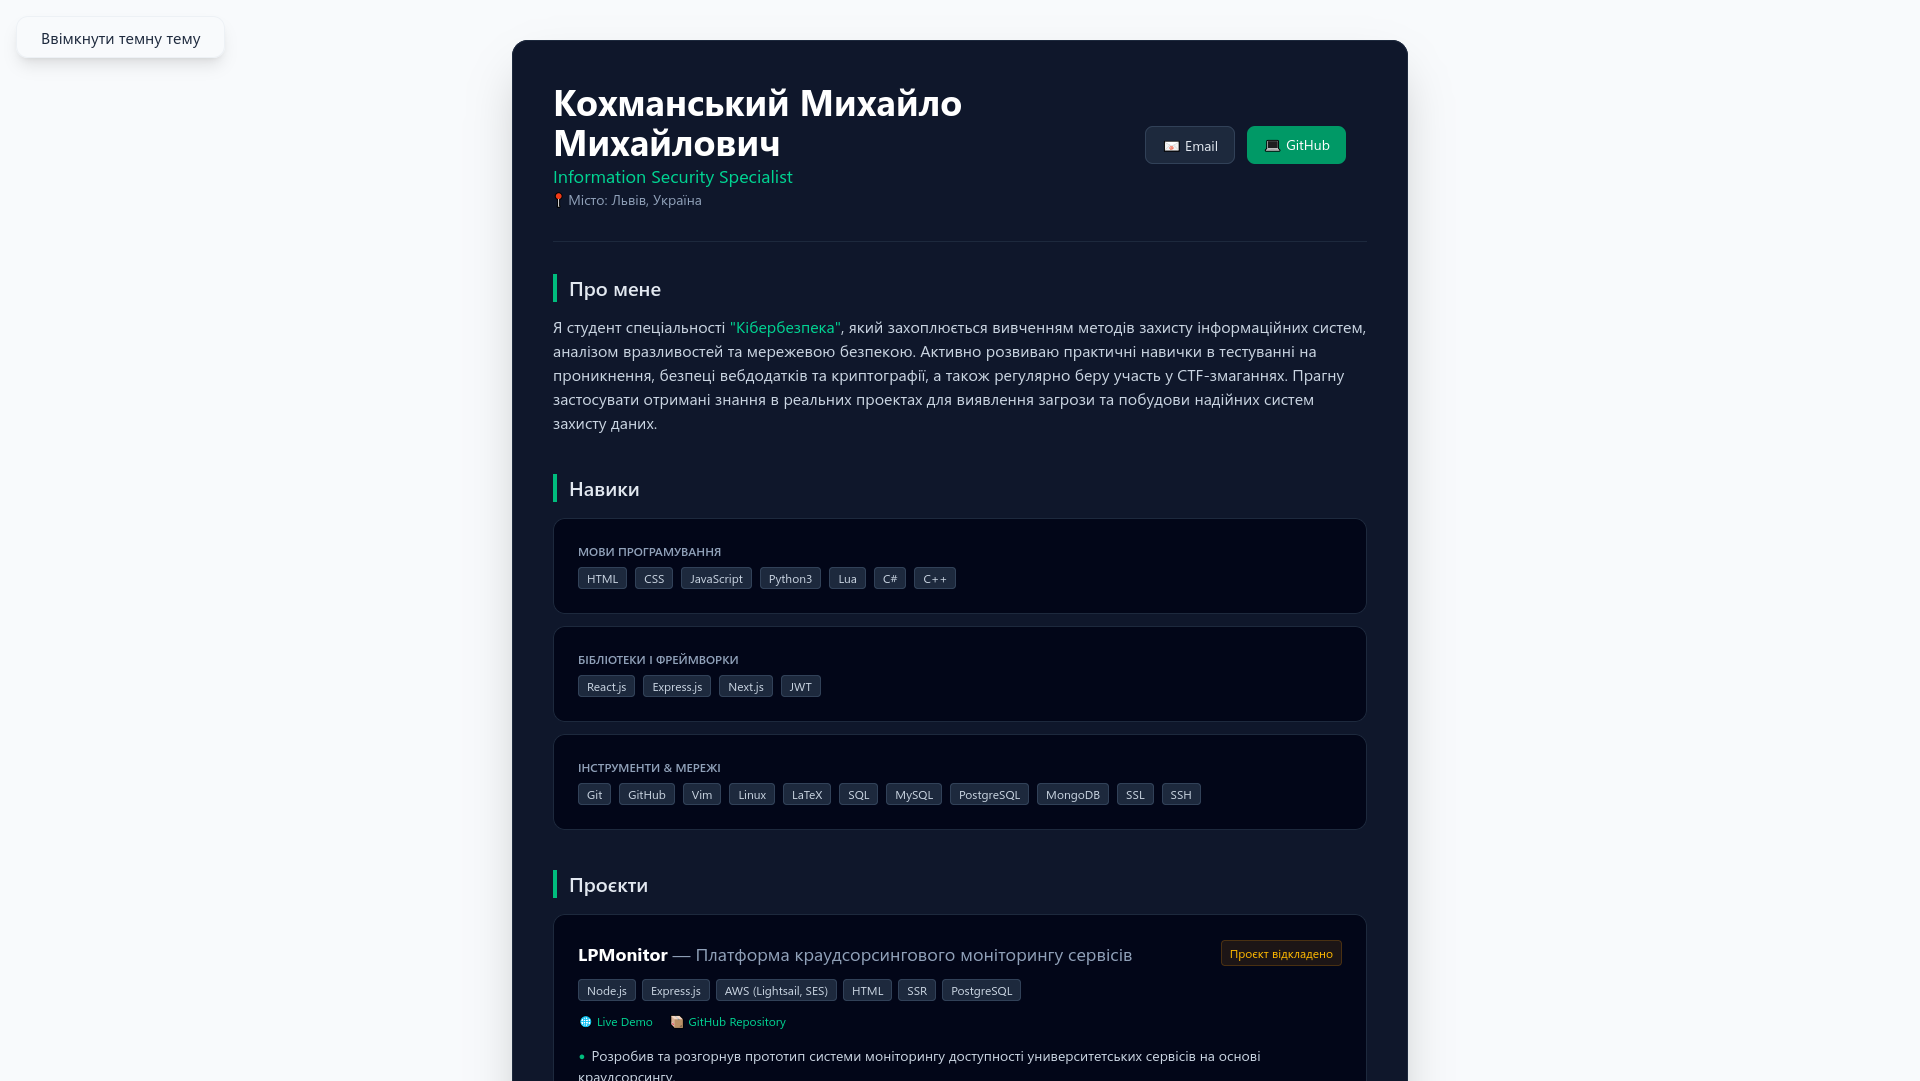
\includegraphics[width=0.7\textwidth]{result_light.png}
	\caption{Вигляд сторінки з світлою темою}
\end{figure}
\section{Висновки}
У ході лабораторної роботи було засвоєно базові концепції JavaScript, опановано управління потоком виконання програми та розглянуто основи взаємодії JavaScript із HTML, а також застосовано здобуті знання у середовищі React шляхом реалізації аналогічного функціоналу за допомогою сучасних хуків (\verb|useState|, \verb|useEffect|) та компонентів у проєкті \verb|lab_2_react|.
\end{document}

